\documentclass[report]{jlreq}
\usepackage{global}
\usepackage{./local}
\subfiletrue
\def\assetspath{../}
%\makeindex
\chead{2007}
\begin{document}

% ------------------------------------------------------------
%
% ------------------------------------------------------------
\section{A}

\begin{problem}[第1問]
    $A$を行列
    \begin{equation}
        A =
            \begin{pmatrix}
                2 & 1 & 1 \\
                -1 & 2 & -1 \\
                -1 & -1 & 0
            \end{pmatrix}
    \end{equation}
    とする。以下の問いに答えよ。
    \begin{enumerate}
        \item $A$の固有値および広義固有空間を全て求めよ。
        \item $AB = 2BA$を満たす任意の3次正方行列$B$は$B^3 = O$を満たすことを示せ。
        \item $AB = 2BA$を満たす零行列でない3次正方行列$B$を1つ求めよ。
    \end{enumerate}
\end{problem}

\begin{answer}
    \uline{(1 略解)} \quad
    固有多項式は$\det (XI - A) = (X - 1)^2 (X - 2)$となる。
    固有値は$1, 2$である。
    固有値$\lambda$に関する広義固有空間を$V_{[\lambda]}$と書くことにすれば
    \begin{equation}
        V_{[2]} = \C \begin{pmatrix} 1 \\ 1 \\ -1 \end{pmatrix},
            \quad
            V_{[1]}
                = \C \begin{pmatrix} 1 \\ 0 \\ -1 \end{pmatrix}
                + \C \begin{pmatrix} 0 \\ 1/2 \\ 1/2 \end{pmatrix}
    \end{equation}
    となる。
    \begin{equation}
        P \coloneqq \begin{pmatrix}
            1 & 1 & 0 \\
            1 & 0 & 1/2 \\
            -1 & -1 & 1/2
        \end{pmatrix},
            \quad
            J \coloneqq \begin{pmatrix}
                2 & 0 & 0 \\
                0 & 1 & 1 \\
                0 & 0 & 1
            \end{pmatrix}
    \end{equation}
    とおくと$AP = PJ$が成り立つ。

    \uline{(2)} \quad
    $AB = 2BA$の成立を仮定すると、両辺の$\det$をとって
    $\det A \det B = 8 \det B \det A$となるから、
    $\det A \neq 0$であることとあわせて
    $\det B = 8 \det B$、したがって$\det B = 0$を得る。
    もし$B^3 \neq O$なら
    両辺の$\det$をとって$(\det B)^3 \neq 0$、
    したがって$\det B \neq 0$となり矛盾が生じる。
    したがって$B^3 = O$である。

    \uline{(3)} \quad
    $AB = 2BA$より
    $JP^{-1}BP = 2P^{-1}BPJ$だから、
    $P^{-1}BP \eqqcolon \begin{pmatrix}
        a & b & c \\
        d & e & f \\
        g & h & i
    \end{pmatrix} \in M_3(\C)$とおくと
    とおくと
    \begin{equation}
        \begin{pmatrix}
            2a & 2b & 2c \\
            d+g & e+h & f+i \\
            g & h & i
        \end{pmatrix}
            = 2 \begin{pmatrix}
                2a & b & b+c \\
                2d & e & e+f \\
                2g & h & h+i
            \end{pmatrix}
    \end{equation}
    を得る。
    直接計算により$P^{-1}BP = \begin{pmatrix}
        0 & 0 & c \\
        0 & 0 & 0 \\
        0 & 0 & 0
    \end{pmatrix}$を得る。
    そこで$c = 1$とおけば
    $B
        = P \begin{pmatrix}
            0 & 0 & 1 \\
            0 & 0 & 0 \\
            0 & 0 & 0
        \end{pmatrix} P^{-1}
        = \begin{pmatrix}
            2 & 0 & 2 \\
            2 & 0 & 2 \\
            -2 & 0 & -2
        \end{pmatrix}$
    を得る。
    定め方からこの$B$は$AB = 2BA$を満たす。
\end{answer}

\begin{problem}[第2問]
    $\R$ 上の関数$f(x,y)$を$f(0,0) = 0$、
    原点以外で$f(x,y) = \frac{x^3 - y^3}{x^2 + y^2}$と定義する。次の問いに答えよ。
    \begin{enumerate}
        \item $f(x,y)$は$\R^2$上連続かつ1回偏微分可能であることを示せ。
        \item $f(x,y)$は$\R^2$上全微分可能かどうか、理由をつけて答えよ。
        \item $D = \{(x,y) \in \R^2 \mid x^2 + y^2 < 1, f(x,y) > 0\}$とおくとき、積分
            \begin{equation}
                I = \iint_D \frac{\sin f(x,y)}{f(x,y)} dxdy
            \end{equation}
            の値を求めよ。
    \end{enumerate}
\end{problem}

\begin{answer}
    \uline{(1)} \quad
    原点以外での連続性は$f$の定義式より直ちに従う。
    原点での連続性は
    $\lim_{\substack{(x, y) \to (0, 0) \\ (x, y) \neq (0, 0)}} f(x, y) = 0$
    をいえばよい。
    ここで$(x, y) \neq (0, 0)$のとき
    \begin{equation}
        f(x, y)
            = \frac{x^3 - y^3}{x^2 + y^2}
            = (x - y) \myparen{
                1 + \frac{xy}{x^2 + y^2}
            }
    \end{equation}
    である。
    したがって任意の$\eps > 0$に対し、
    $\delta \coloneqq \eps / 3$とおけば、
    $\| (x, y) - (0, 0) \| < \delta$なる
    すべての$(x, y) \in \R^2 \setminus \{(0, 0)\}$に対し
    \begin{alignat}{1}
        \left|
            \frac{x^3 - y^3}{x^2 + y^2}
        \right|
            &= |x - y| \left|
                1 + \frac{xy}{x^2 + y^2}
            \right| \\
            &\le (|x| + |y|) \myparen{
                1 + \left| \frac{xy}{x^2 + y^2} \right|
            } \\
            &\le (|x| + |y|) \myparen{
                1 + \frac{1}{2}
            }
                \quad
                (\text{AM-GM}) \\
            &\le 2 \| (x, y) \| \cdot \frac{3}{2} \\
            &= 3 \| (x, y) \| \\
            &< 3 \delta \\
            &= \eps
    \end{alignat}
    を得る。
    よって
    $\lim_{\substack{(x, y) \to (0, 0) \\ (x, y) \neq (0, 0)}} f(x, y) = 0$
    がいえた。
    したがって$f$は原点で連続である。
    よって$f$は$\R^2$上連続である。

    つぎに$f$が$\R^2$上1回偏微分可能であることを示す。
    原点以外での1回偏微分可能性は$f$の定義式より直ちに従う。
    あとは原点での1回偏微分可能性を考えればよい。
    $x, y$それぞれに関して
    \begin{alignat}{2}
        \lim_{\substack{t \to 0 \\ t \neq 0}}
            \frac{f(t, 0) - f(0, 0)}{t}
            &= \lim_{\substack{t \to 0 \\ t \neq 0}}
                \frac{t^3}{t^3}
            &&= 1 \\
        \lim_{\substack{t \to 0 \\ t \neq 0}}
            \frac{f(0, t) - f(0, 0)}{t}
            &= \lim_{\substack{t \to 0 \\ t \neq 0}}
                \frac{-t^3}{t^3}
            &&= -1
    \end{alignat}
    という極限が存在するから、
    偏微分の定義より$f$は原点で$x, y$それぞれに関し1回偏微分可能である。

    \uline{(2)} \quad
    $f$は$\R^2$上全微分可能ではないことを背理法で示す。
    そこで$f$が$\R^2$上全微分可能であると仮定すると、
    とくに原点で全微分可能であり、
    原点における$f$の1次近似$p(x, y)$が存在し
    \begin{alignat}{1}
        &p(x, y)
            = f(0, 0) + \deldel[f]{x}(0, 0) x + \deldel[f]{y}(0, 0) y
            = x - y \\
        &\lim_{\| (x, y) \| \to 0}
            \frac{f(x, y) - p(x, y)}{\| (x, y) \|}
            = 0
            \locallabel{eq:limit}
    \end{alignat}
    をみたす。
    一方
    $\theta \in (0, \pi / 4)$をひとつ選べば、
    いかなる$\delta > 0$に対しても、
    $(x, y)
        \coloneqq \myparen{
            \frac{\delta}{2} \cos \theta,
            \frac{\delta}{2} \sin \theta
        }
        \in \R^2 \setminus \{(0, 0)\}$
    は$\| (x, y) \| = \frac{\delta}{2} < \delta$でありながら
    \begin{equation}
        \left| \frac{f(x, y) - p(x, y)}{\| (x, y) \|} \right|
            = \left| \frac{(x - y) xy}{(x^2 + y^2)^{3/2}} \right|
            = \left|
                (\cos \theta - \sin \theta)
                \cos \theta \sin \theta
            \right|
    \end{equation}
    となり、
    右辺は$\delta$によらない正定数だから
    \localcref{eq:limit}に矛盾する。
    背理法より$f$は$\R^2$上全微分可能でない。

    \uline{(3)} \quad
    $D$は下図の塗りつぶされた部分 (境界を除く) である。
    \begin{center}
        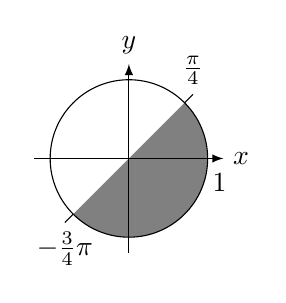
\begin{tikzpicture}
            \fill[gray] (-135:1) arc (-135:45:1) -- (0,0) -- cycle;
            \draw (0,0) circle (1);
            
            % Draw x-axis and label
            \draw[-latex] (-1.2,0) -- (1.2,0) node[right] {$x$};
            \node at (1.15, -0.3) {$1$};
            
            % Draw y-axis and label
            \draw[-latex] (0,-1.2) -- (0,1.2) node[above] {$y$};
            
            % Draw labels for intersections
            \draw (45:1) -- (45:1.15) node[above] {$\frac{\pi}{4}$};
            \draw (-135:1) -- (-135:1.15) node[below] {$-\frac{3}{4}\pi$};
        \end{tikzpicture}
    \end{center}
    そこで極座標に変数変換して積分を計算すれば
    \begin{alignat}{1}
        I
            &= \int_D f(x, y) \, dx dy \\
            &= \int_{r = 0}^1 \int_{\theta = -\frac{3}{4}\pi}^{\frac{\pi}{4}}
                r^2 (\cos \theta - \sin \theta) \, d\theta dr \\
            &= \frac{2}{3} \sqrt{2}
    \end{alignat}
    を得る。
\end{answer}

\begin{problem}[第3問]
    $A, B$を$\R$のコンパクトな部分集合、
    $U$を$\R^2$の開集合であって$A \times B \subset U$なるものとする。
    このとき、$\R$の開集合$V, W$であって
    $A \times B \subset V \times W \subset U$
    をみたすものが存在することを示せ。
\end{problem}

\begin{answer}
    $A, B$は$\R$のコンパクト部分集合だから
    $A \times B$は$\R^2$のコンパクト部分集合である。
    いま$\{ U \}$は$\R^2$における$A \times B$の開被覆であるから、
    Lebesgue 数の補題より
    ある$\delta > 0$が存在して、
    任意の$(a, b) \in A \times B$に対し
    $(a, b)$の$\R^2$における$\delta$-近傍$B_\delta (a, b)$は
    $U$に含まれる。
    ここで$\R$の開集合$V, W$を
    $V \coloneqq \bigcup_{a \in A} B_{\delta / 2}(a), \;
        W \coloneqq \bigcup_{b \in B} B_{\delta / 2}(b)$
    で定める。
    これらが求める$V, W$であることを示す。
    まず$A \subset V, \; B \subset W$より
    $A \times B \subset V \times W$が成り立つ。
    つぎに$(v, w) \in V \times W$とすると、
    $V, W$の定義よりある$a \in A, \; b \in B$が存在して
    $v \in B_{\delta / 2}(a), \; w \in B_{\delta / 2}(b)$が成り立つ。
    したがって
    \begin{alignat}{1}
        \| (v, w) - (a, b) \|^2
            &\le (v - a)^2 + (w - b)^2 \\
            &< \myparen{\frac{\delta}{2}}^2 + \myparen{\frac{\delta}{2}}^2 \\
            &= \frac{\delta^2}{2} \\
            &< \delta^2 \\
        \therefore \quad \| (v, w) - (a, b) \|
            &< \delta
    \end{alignat}
    を得る。
    よって$(v, w) \in B_\delta (a, b) \subset U$である。
    したがって$V \times W \subset U$もいえた。
\end{answer}



% ------------------------------------------------------------
%
% ------------------------------------------------------------
\section{B}

\begin{problem}[第10問]
    集合 $X$ 上の$\sigma$-加法族を$\mathcal{B}$とし、
    $\mathcal{B}$上定義された二つの測度$\mu, \nu$を考える。
    $\mathcal{B}$の全ての元$A$に対して、$\mu(A) \ge \nu(A)$であるとする。
    このとき、$\mathcal{B}$の各元$A$に対して、$\lambda(A)$を
    \begin{equation}
        \lambda(A) =
            \sup\{\mu(B) - \nu(B) \mid \nu(B) < +\infty, B \subset A, B \in \mathcal{B}\}
    \end{equation}
    と定める。このとき、
    \begin{enumerate}
        \item $\nu$が有限測度のとき、
            $\lambda$は$\mathcal{B}$上定義された測度となり、
            $\mathcal{B}$の全ての元$A$に対して、
            $\mu(A) = \nu(A) + \lambda(A)$が成り立つことを示せ。
        \item $\nu$が有限とは限らない測度であっても、
            $\lambda$は$\mathcal{B}$上定義された測度となり、
            $\mathcal{B}$の全ての元$A$に対して、
            $\mu(A) = \nu(A) + \lambda(A)$が成り立つことを示せ。
    \end{enumerate}
\end{problem}

\begin{answer}
    
\end{answer}

\end{document}